\problemname{Flatland Olympics}
\providecommand{\maxn}{10^{}}%
\renewcommand{\maxn}{10^{5}}%
\providecommand{\maxd}{10^{}}%
\renewcommand{\maxd}{10^{9}}%
\providecommand{\dysonCompany}{}%
\renewcommand{\dysonCompany}{Dy~\&~Son}%
\illustration{.4}{usain_bolt_winning_cropped}{\href{https://en.wikipedia.org/wiki/File:Usain_Bolt_winning.jpg}{2008 Beijing Olympics} by PhotoBobil}%
It is the day after Olympia, and you---as the organizer---are happy that \emph{everything} worked well in these troublesome times.
Well, not everything\dots.

Since this morning e-mails have been filling up your inbox, containing complaints about obscured views during the most important race: the \mbox{$100$-meter} dash.
They demand their money back, or threaten exposing you on social media.
To make things worse, spectators have not just complained once, but they have sent you a separate e-mail for every person that blocked their view at some point during the race!
They even wrote multiple e-mails when two or more people blocked their view at the same time.
And not only that, some visitors complained to the main sponsor \emph{\dysonCompany{}} who in turn has urged you to improve the situation. 

Since you expect that a greater number of visitors will be allowed to spectate at the next Olympic games, you assume that there will be even more complaints if you do not address this issue.
If the situation will be too bad, you may even lose your sponsor \dysonCompany{}.
Therefore, you decide to count the number of complaints beforehand.
To do this, you model the running track as a straight line segment, and count the maximal number of complaints you could get based on the seating of the visitors.
Depending on the number of complaints you expect, you will determine if you need to rework the seating or just reconfigure your spam blocker and try to find a new sponsor.

\begin{Input}
	The input consists of:
	\begin{itemize}
        % Force this item to be on the same page as the start of the Input section.
        \begin{samepage}
        \item One line containing four integers $x_s$, $y_s$, $x_e$ and $y_e$ $(|x_s|, |y_s|, |x_e|, |y_e| \leq\maxd)$, where $s=(x_s, y_s)$ is the starting point of the running track and $e=(x_e, y_e)$ is the end point of the running track. Both $s$ and $e$ belong to the running track.
        \end{samepage}
        \item One line containing an integer $n$ $(1 \leq n \leq \maxn)$, the number of visitors.
        \item $n$ lines, each containing two integers $x$ and $y$ $(|x|,|y|\leq\maxd)$, where $(x,y)$ is the location of the seat of a visitor.
	\end{itemize}
	It is guaranteed that the track has a positive length, i.e.\ $s\neq e$.
	Further, you can assume that all visitors are seated at distinct locations and that no visitor is seated on the track.
\end{Input}

\begin{Output}
	Output the total number of complaints that you would receive for the given seating.
\end{Output}

\begin{figure}[!h]
	\centering
	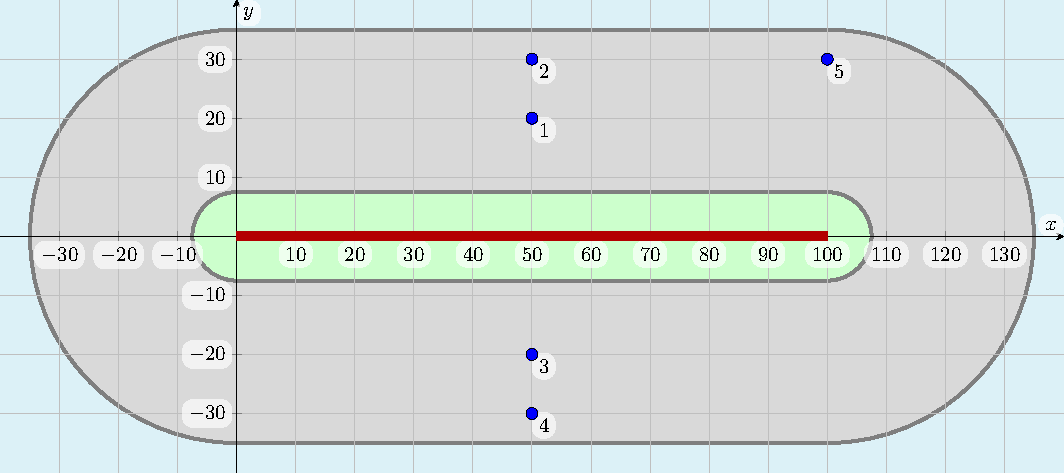
\includegraphics[width=0.7\textwidth]{sample2}
	\caption{Illustration of Sample Input 2.
		The running track is drawn as a red line and the seats of the visitors are highlighted in blue.
		The second visitor will complain about the first visitor and the fourth visitor will complain about the third visitor.}
\end{figure}
